% Copyright (C) Dean Gadberry - All Rights Reserved
% Unauthorized copying of this file, via any medium is strictly prohibited
% Proprietary and confidential
% Written by Dean Gadberry <dean@deangadberry.com>, 2023

\documentclass[12pt,a4paper,english]{article}
\renewcommand{\familydefault}{\sfdefault}
\usepackage{sectsty}        % allow redefinition of section command formatting
    \allsectionsfont{\normalsize}
\usepackage[centering,noheadfoot,margin=1in]{geometry}
\usepackage{lipsum}
\setlength{\parindent}{0em}
\usepackage{hanging}

% code pasting
\usepackage{listings}

\usepackage{circuitikz}

\usepackage{graphicx}
\graphicspath{ {./images/} }

% https://tex.stackexchange.com/questions/8845/how-to-move-page-number
\usepackage{fancyhdr}
\fancyhf{} % clear all header and footers
\renewcommand{\headrulewidth}{0pt} % remove the header rule
\rfoot{\thepage}

% https://tex.stackexchange.com/questions/30720/footnote-without-a-marker
\newcommand\blindfootnote[1]{
  \begingroup
  \renewcommand\thefootnote{}\footnote{#1}
  \addtocounter{footnote}{-1}
  \endgroup
}
\AtEndDocument{\blindfootnote{\textrm{This document proudly made using \LaTeX{}}}}

\pagestyle{fancy}
\begin{document}
Dean Gadberry

NCTC COSC 2425 S23

3/25/23
\section*{\centering{ Exam 1 - Chapters 1 - 4 \& Notes}}
\begin{enumerate}
\item What is 23(base6) minus 23(base4)? Express the answer in base 10.

23_6 = 3(6^0) + 2(6^1) = 3+12 = 15_{10}
    
23_4 = 3(4^0) + 2(4^1) = 3+8 = 11_{10}

15 + 11 = 26_{10}
 
\item  Find the value of the following 8-bit two's complement binary number:
    11001010
\begin{lstlisting}
    11001010 - 1 = 11001001
         Inversion 00110110
    00110110 = 2^1 + 2^2 + 2^4 + 2^5 = 2+4+16+32 = 54

    11001010 = -54
\end{lstlisting}
\item  Using the Hamming Algorthm with EVEN parity, find the position of the error and the corrected data string.
    
\begin{lstlisting}
    1001 0001 0010

         100100010010
    p1 = ? 0 0 0 0 1  = 1
    p2 =  ?0  00  01  = 1
    p3 =    ?000    0 = 0
    p4 =        ?0010 = 1
         12 4   8
         100100010010
         11 0   1     
         *X X   *     = 6

    bit 6 incorrect
              _
         100101010010
    p1 = ? 0 0 0 0 1  = 1
    p2 =  ?0  10  01  = 0
    p3 =    ?010    0 = 1
    p4 =        ?0010 = 1

         12 4 _ 8
         100101010010
         10 1   1

    Position of error -> 6
    Corrected Data String -> 1001 0101 0010
      \end{lstlisting}

\item List all the ordered pairs that make the following expression true:

   ¬(¬A + ¬B)

    ¬¬A * ¬¬B       DeMorgan's 

    A * B       Double Negation

    The ordered pair that makes this espression true is 
        (1,1)

  \begin{lstlisting}
     A    B    Value
     0    0    0
     1    0    0
     0    1    0
     1    1    1
   \end{lstlisting}

\item Write the Boolean expression in Sum of Product (SOP) form represented by the truth table below

\begin{tabular}{c | c | c | c }
 \hline
 A & B & C & Output \\ [0.5ex] 
 \hline
 0 & 0 & 0 & 0 \\
 0 & 0 & 1 & 1 \\
 0 & 1 & 0 & 0 \\
 0 & 1 & 1 & 1 \\
 1 & 0 & 0 & 1 \\
 1 & 0 & 1 & 0 \\
 1 & 1 & 0 & 1 \\
 1 & 1 & 1 & 1 \\
\end{tabular}

\item Write the simplified (minimized) expression for the boolean function defined by the following Karnaugh Map (KMap) in Sum of Product (SOP) form.
  
  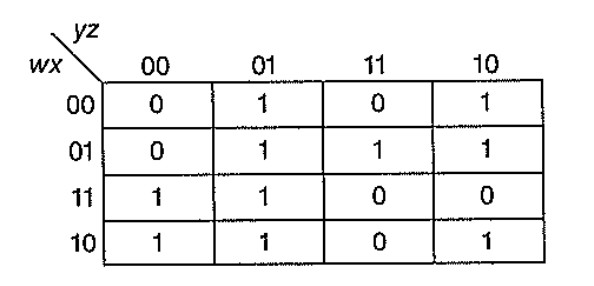
\includegraphics[scale=.5]{karnaughmap}

\item What is the Boolean Expression represented by the digital circuit?

  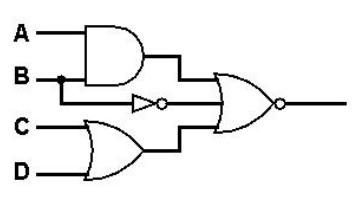
\includegraphics[scale=.5]{logiccircuit}
\lnot[(A * B) + \lnot B + (C + D)]

\item Draw the circuit diagram for the following expression:

  (A\oplus B) + \lnot(\lnot B * C)

  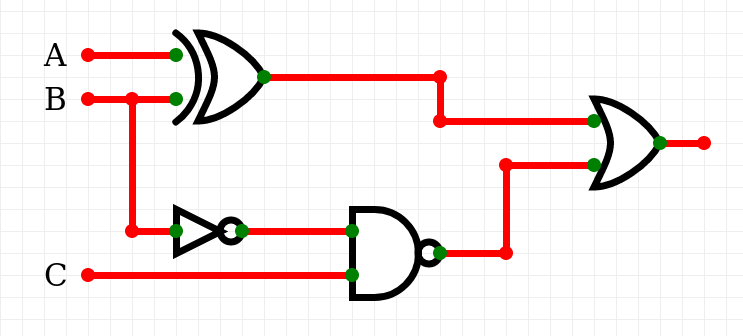
\includegraphics[scale=.5]{logicdrawing}

\item What is the final value of C when the program is run?
  \begin{lstlisting}

    A   DC      4       # label A defined as 4
    B   DC      120     # label B defined as 120
    C   DC      0       # label C defined as 0
    TOP LOAD    C       # C in the accumulator
        ADD     =1      # ACC += 1
        STORE   C       # C = 1
        LOAD    C       # C in ACC
        SUB     A       # ACC = 1 - 4 = -3
        SUB     A       # ACC = -3 - 4 = -7
        SUB     A       # ACC = -7 - 4 = -11
        STORE   B       # B = -11
        LOAD    B       # ACC = -11
        SUB     A       # ACC = -11 - 4 = -15
        BG      TOP     # Does not Branch to TOP because !(ACC>0)
        END             # END 

    The final value of C is 1

\end{lstlisting}

\end{enumerate}
\end{document}
